\documentclass[letterpaper,12pt]{article}
\usepackage{tabularx} % extra features for tabular environment
\usepackage{amsmath}  % improve math presentation
\usepackage{tcolorbox}
\usepackage{graphicx} % takes care of graphic including machinery
\usepackage{subfig}
\usepackage[margin=1in,letterpaper]{geometry} % decreases margins
\usepackage[final]{hyperref} % adds hyper links inside the generated pdf file
\usepackage[utf8]{inputenc}
\hypersetup{
	colorlinks=true,       % false: boxed links; true: colored links
	linkcolor=blue,        % color of internal links
	citecolor=blue,        % color of links to bibliography
	filecolor=magenta,     % color of file links
	urlcolor=blue         
}

\usepackage{fancyhdr}
\usepackage{lastpage}
 
\pagestyle{fancy}
\fancyhf{}
\renewcommand{\headrulewidth}{0pt}

% footer
\lfoot{SF1900}
\cfoot{KTH}
\rfoot{\thepage \hspace{1pt} / \pageref{LastPage}}

\begin{document}

\title{
    \textbf{Lab 1}\\
    \large{SF1900 - Probability Theory and Statistics}
    }
\author{Simone Stefani}
\date{Fall Term 2017}
\maketitle
\thispagestyle{fancy}

\section*{Introduction}
This is the instructions for computer exercise 1, please bring a printed copy to computer exercise 1. Please read the instructions carefully, and make sure that you understand what the MATLAB code included does. The computer exercise is pass/fail. In order to pass you first have to be able to present written solutions to the preparatory exercises. Each student should have prepared solutions \textbf{individually}. For the computer exercise it is allowed to work in groups of \textbf{at most two} persons per group. If you pass the computer exercise you will be given 3 bonus points at the written exam Wednesday October 26 2016, \textbf{given that you at the exam obtain at least 20 points without the bonus points}.

\section*{Preparatory exercises}
\begin{enumerate}
  \item Consider a continuous random variable $X$. For this random variable write down the definition of the cumulative distribution function and the density function, and the relationship between the two.
  \item Suppose that the random variable $X$ has a density function of the following form
  \begin{equation}
  f_{X}(x) = \lambda e^{-\frac{x}{\lambda}} + \frac{\lambda}{x}, \quad x \in [1,10]
  \end{equation}
  where $\lambda$ is a real number.
  
  \begin{enumerate}
    \item Determine (approximately) the value of $\lambda$ that makes $f_{X}$ a density function.
    \begin{tcolorbox}
    \textbf{Answer:}
    Compute the distribution function $F_{X}(x)$:
    \begin{equation*}
    F_{X}(x) = \int_{1}^{10} \lambda e^{-\frac{x}{\lambda}} + \frac{\lambda}{x} dx = \lambda (\lambda e^{-\frac{10}{\lambda}} (e^{\frac{9}{\lambda}}-1) + ln(10))
    \end{equation*}
    In order for $F_{X}(x)$ to be a distribution function it must equal to $1$:
    \begin{equation*}
    \lambda (\lambda e^{-\frac{10}{\lambda}} (e^{\frac{9}{\lambda}}-1) + ln(10)) = 1 \quad \lambda \approx 0.426704
    \end{equation*}
    \end{tcolorbox}
    
    \item Determine the cumulative distribution function of $X$.
    \begin{tcolorbox}
    \textbf{Answer:}
    The cumulative distribution function can be expressed as:
    \begin{gather*}
        F_{X}(x) = F_{X}(b) - F_{X}(a) = P(a < X \leq b)\\
        = \int_{a}^{b} 0.4267 e^{-\frac{x}{0.4267}} + \frac{0.4267}{x} dx \quad with \quad 1 \leq a < b \leq 10
    \end{gather*}
    \end{tcolorbox}
    
    \item Determine the probability that $X$ is less than 7. Use the value $\lambda = 0.4267$.
    \begin{tcolorbox}
    \textbf{Answer:}
    The probability $P(X \leq 7)$ can be computed as the cumulative distribution between 1 and 7:
    \begin{gather*}
    P(X \leq 7) = F_{X}(7) - F_{X}(1) = \int_{1}^{7} 0.4267 e^{-\frac{x}{0.4267}} + \frac{0.4267}{x} dx = 0.847796
    \end{gather*}
    \end{tcolorbox}
    
    \item Compute $E[X]$.
    \begin{tcolorbox}
    \textbf{Answer:}
    The expectation $E[X]$ for can be computed as:
    \begin{gather*}
    E[X] = \int_{1}^{10} x \left (0.4267 e^{-\frac{x}{0.4267}} + \frac{0.4267}{x} \right ) dx = 3.86523 
    \end{gather*}
    \end{tcolorbox}
  \end{enumerate}
  
  \item Let $U$ be uniformly distributed over the interval $[0, 2\pi]$, and compute
  \begin{enumerate}
    \item $E[\cos(U)]$
    \begin{tcolorbox}
    \textbf{Answer:}
     If $U$ is continuous, then the expectation of $\cos(U)$ is defined as
    \begin{gather*}
    E(\cos(U)) = \int_{0}^{2\pi} \cos(u) f(u) du
    \end{gather*}
    where f is the probability density function $f_{U}(u) = \frac{1}{2\pi - 0}$. Hence:
    \begin{gather*}
    E(\cos(U)) = \int_{0}^{2\pi} \frac{1}{2\pi} \cos(u) du = 0
    \end{gather*}
    \end{tcolorbox}
    
    \item $E[\sin(U)^{2}]$
    \begin{tcolorbox}
    \textbf{Answer:}
    With the same reasoning as above we can compute:
    \begin{gather*}
    E(\sin^{2}(U)) = \int_{0}^{2\pi} \frac{1}{2\pi} \sin^{2}(u) du = \frac{1}{2} = 0.5
    \end{gather*}
    \end{tcolorbox}
  \end{enumerate}
  
  \item State and explain the contents of the Law of Large Numbers (LLN).
    \begin{tcolorbox}
    \textbf{Answer:}
    a \textbf{law of large numbers} is one of several theorems expressing the idea that as the number of trials of a random process increases, the percentage difference between the expected and actual values goes to zero.
    
    Let $X_{1}, X_{2}, ..., X_{n}$ be an independent trials process, with finite expected value $\mu = E(X_{j})$. Then for any $\epsilon > 0$
    \begin{equation*}
        P\left( \left| \frac{1}{n} \sum_{i=1}^{n} X_{i} - \mu \right | < \epsilon \right) \rightarrow 1
    \end{equation*}
    \end{tcolorbox}
  \item  State and explain the contents of the Central Limit Theorem (CLT).
    \begin{tcolorbox}
    \textbf{Answer:}
    the \textbf{central limit theorem} states that the sampling distribution of the mean of any independent, random variable will be normal or nearly normal, if the sample size is large enough.
    If $X_{1}, X_{2}, ...$ is an infinite sequence of independent identically distributed rv's, each with expectation $m$ and standard deviation $\sigma > 0$, and if we set
    \begin{equation*}
        Y_{n} = X_{1}, ... X_{n}
    \end{equation*}
    then we have
    \begin{equation*}
        P\left( a < \frac{Y_{n} - nm}{\sigma \sqrt{n}} < b\right) \rightarrow \Phi(b) - \Phi(a) \quad as \quad n \rightarrow \infty
    \end{equation*}
    \end{tcolorbox}
\end{enumerate}

\section*{Purpose and further introduction}
Start by downloading the following files
\begin{enumerate}
    \item \texttt{plot\_mvnpdf.m}
    \item \texttt{hist\_density.m}
    \item \texttt{birth.dat}
    \item \texttt{birth.txt} - description of the data birth.dat
\end{enumerate}
from the homepage of the course. Make sure the files are downloaded to
the directory you will be working in. To make sure the files are in the right directory type ls to list the files in the current working directory. You can write your commands directly at the prompt in MATLAB, but usually it is easier to work in the editor. If the editor is not open you can open it and create a new file by typing \texttt{edit lab1.m}. The code included below is written in sections. A new section is begun by typing two percent signs. The code \texttt{Ctrl+Enter} executes the commands in a section.\\
\\
The theme for this computer exercise is simulation. In the part of the course which treats probability theory you will learn how to compute different quantities, such as probabilities, expected values etc., given a certain random distribution. For more complicated random models it can be very time consuming, or even impossible to do exact computations.\\
\\
In such circumstances simulation can be an alternative. You then use a computer to simulate outcomes from a certain distribution, and then you can use for instance the mean of the outcomes to estimate the expected value, or some empirical quantile to estimate a probability. In this computer exercise we will do this for some rather simple problems (where explicit computations are possible), but the same basic principles can be applied to more difficult problems where explicit computations are not possible.

\subsection*{Problem 0 - Computing probabilities}
Read the help-files of the functions \texttt{binocdf}, \texttt{binopdf}, \texttt{normcdf}, \texttt{normpdf}, \texttt{expcdf} and \texttt{exppdf}.\\
Let $X_{1} \in Bin(10, 0.3)$, $X_{2} \in N(5, 3)$, and $X_{3} \in Exp(7)$, and compute (using the above mentioned functions) for $k = 1, 2, 3$, i.e. for each of the random variables $X_{1}$, $X_{2}$, and $X_{3}$

\begin{enumerate}
    \item $P(X_{k} \leq 3)$
    \begin{tcolorbox}
    \textbf{Answer:}
    \begin{gather*}
        P(X_{1} \leq 3) = 0.6496 \quad
        P(X_{2} \leq 3) = 0.2525 \quad
        P(X_{3} \leq 3) = 0.3486
    \end{gather*}
    \end{tcolorbox}
    
    \item $P(X_{k} \geq 7)$
    \begin{tcolorbox}
    \textbf{Answer:}
    \begin{gather*}
        P(X_{1} \geq 7) = 0.0016 \quad
        P(X_{2} \geq 7) = 0.2525 \quad
        P(X_{3} \geq 7) = 0.3679
    \end{gather*}
    \end{tcolorbox}
    
    \item $P(3 < X_{k} \leq 4)$
    \begin{tcolorbox}
    \textbf{Answer:}
    \begin{gather*}
        P(3 < X_{1} \leq 4) = 0.2001 \quad
        P(3 < X_{2} \leq 4) = 0.1169 \quad
        P(3 < X_{3} \leq 4) = 0.0867
    \end{gather*}
    \end{tcolorbox}
\end{enumerate}

\subsection*{Problem 1 - Probability density functions}
Plot the density function of an exponentially distributed random variable
with expectation $\mu$. Now do the same thing for the density function you worked with in the preparatory exercise 2. Discuss the differences between the two distributions.

\begin{figure}
    \subfloat[Simple exponential distribution]{{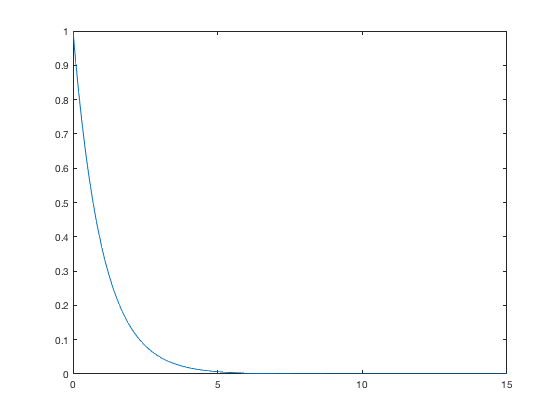
\includegraphics[width=8cm]{img/pb_1b.png} }}
    \quad
    \subfloat[Distribution from prep. ex. 2]{{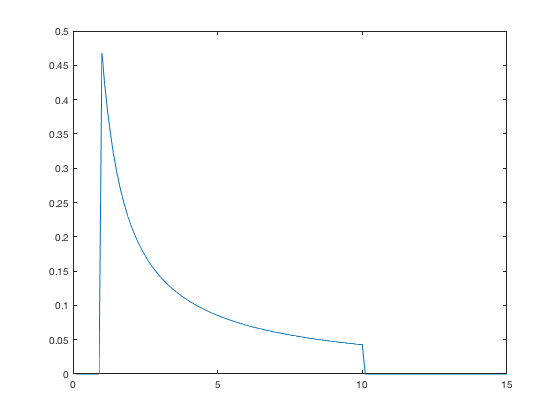
\includegraphics[width=8cm]{img/pb_1a.png} }}
    \label{fig:example}
\end{figure}
\begin{tcolorbox}
\textbf{Comment:}
the exponential distribution has the density function $\lambda e^{-\lambda x}$. The distribution from exercise has inverted $\lambda $ in the exponent and added $\frac{\lambda}{x}$ to the density function. Thus, in this distribution the rv is approximately exponentially distributed, with a certain shift $\frac{\lambda}{x}$. Moreover the interval is limited in $[1, 10]$.
\end{tcolorbox}

\subsection*{Problem 2 - Multivariate normal distribution}
The multivariate normal distribution can be visualized using \texttt{plot\_mvnpdf}. Investigate what the function does and try some different values for the parameters. How does changing the parameters values affect the plot?
\begin{tcolorbox}
\textbf{Comment:}
the function \texttt{plot\_mvnpdf} plots the density function in two variables $X$ and $Y$. This density function has a two-dimensional normal distribution. The variables \texttt{mux} and \texttt{muy} are respectively $X$ and $Y$ expectations. The variables \texttt{sigmax} and \texttt{sigmay} are respectively $X$ and $Y$ standard deviations. The variable \texttt{rho} is the correlation coefficient between $X$ and $Y$. The values of \texttt{mux} and \texttt{muy} determine the midpoint of the plot. The standard deviations \texttt{sigmax} and \texttt{sigmay} determine the size of the plot in x and y dimensions.
\end{tcolorbox}

\subsection*{Problem 3 - Simulating random numbers}
In this exercise you should generate a large number of random numbers, draw a histogram of the simulated data, and finally plot the true density function in the same figure as the histogram.\\
Please note that the function \texttt{exprnd} in MATLAB takes the expectation $\mu$ as a parameter, just like the textbook. Other textbooks and programs use $\lambda = 1 / \mu$ as the parameter. Redo the simulation and study how the histogram changes. What is the relation between the red line and the histogram, and how would you explain the fluctuations around the red line?
\begin{tcolorbox}
\textbf{Comment:}
the histogram usually follows the red line. Such line is traced as a perfect exponential distribution while the bars of the histogram come from numbers randomly generated but yet with an exponential distribution This is the reason of the deviations between the bars and the line and also why the are slightly different every time we run the script.
\end{tcolorbox}

\subsection*{Problem 4 - LLN, Monte Carlo and CLT}
In this section you should again generate a large number of random numbers. This time they will be used to estimate expectations and probabilities. Suppose that you for some reason are interested in the expected value of the roll of a dice. This is not hard to compute analytically, but you could also imagine throwing the dice a large number of times and take the mean value of the throws. If $X_{1}, X_{2}, ... , X_{n}$ are identically distributed with expectation $\mu$ then according to the law of large numbers in it holds that
\begin{equation*}
    P\left( \left| \frac{1}{n} \sum_{i=1}^{n} X_{i} - \mu \right | < \epsilon \right) \rightarrow 1
\end{equation*}
for every $\epsilon > 0$ when $n \rightarrow \infty$. This means that the probability that the difference between the true value of the expectation and the mean value is less than $\epsilon$ tends to one as the number of observations (in the example above the number of throws) tends to infinity. This approach to estimating expected values is known as a Monte Carlo method.\\
\\
\textit{The idea behind the Monte Carlo method is old and can be found in mathematics from the 18th century, but it was not until the second half of the 20th century, when computers made it possible to do massive amounts of computations, that the modern versions of the method were developed. In the late 1940s Stanislaw Ulam and John von Neumann developed methods to make the “throw of a dice” using a computer. The method has been named after the Monte Carlo Casino in Monaco, and was used in the simulations for the Manhattan Project, a research and development project that produced the first nuclear weapons.}

\subsubsection*{Illustration of the Law of Large Numbers}
The code below simulates $M$ random numbers from an exponential distribution. The mean value of the generated outcomes is plotted as the simulation proceeds. The plot thus shows how your estimate, the mean value of the outcomes, develops as the number of simulated outcomes \texttt{k} increases.\\
If you get tired of waiting you can comment out the row with \texttt{pause} by typing a percent sign at the beginning of the row. Does the plot look the way you expected it to?
\begin{figure}
\centering
    \subfloat[Simple exponential distribution]{{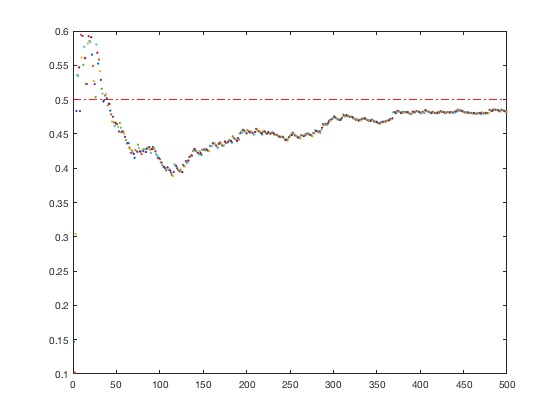
\includegraphics[width=10cm]{img/pb_4a.png} }}
\end{figure}
\begin{tcolorbox}
\textbf{Answer:}
the plot reflects my expectations. The points are quite sparse when the sample is small and they tend to align very closely to the mean value when the sample grows. This is in accordance with the idea that as the number of trials of a random process increases, the percentage difference between the expected and actual values goes to zero.
\end{tcolorbox}

\subsubsection*{Illustration of the Central Limit Theorem}
The code below simulates random numbers from an exponential distribution and then adds them up. Study the code and explain what \texttt{N} represents.
\begin{tcolorbox}
\textbf{Answer:}
the variable \texttt{N} represents the sample size from which we compute the distribution. 
\end{tcolorbox}

Change the value of  \texttt{N}, what happens when you increase and decrease the value, respectively? Why?\\

\begin{tcolorbox}
\textbf{Comment:}
when \texttt{N} becomes grows, going to infinity, the distribution of the sum becomes more like a normal distribution. When $N = 1$, the histogram looks like an exponential distribution. When we increase N then the distribution becomes more "normal". This is the phenomenon described by the CLT. 
\end{tcolorbox}

\begin{figure}
    \subfloat[N = 1]{{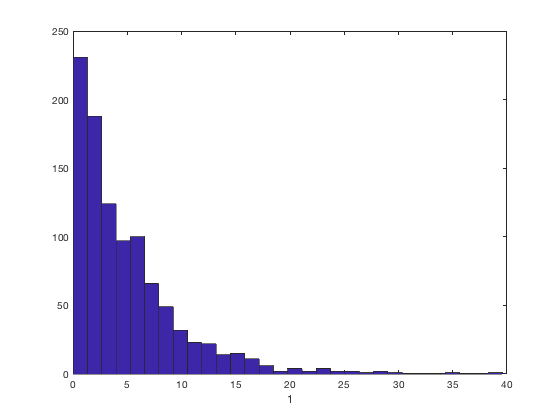
\includegraphics[width=8cm]{img/pb_4b.png} }}
    \quad
    \subfloat[N = 20]{{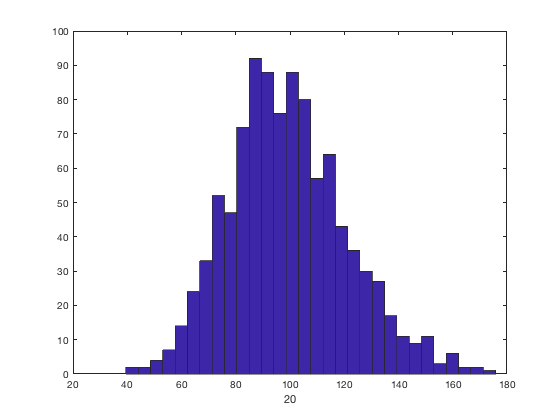
\includegraphics[width=8cm]{img/pb_4c.png} }}
    \label{fig:example}
\end{figure}

For what value of \texttt{N} does it look like there is no change if you increase it further?\\

\begin{tcolorbox}
\textbf{Answer:}
after \texttt{N} = 30 the histogram resembles a normal distribution and does not seem to change if \texttt{N} is increased further.
\end{tcolorbox}

What distribution does the sums appear to have? Why do they have this distribution?\\
\begin{tcolorbox}
\textbf{Answer:}
the sum appear to have a normal (Gaussian) distribution in accordance with the Central Limit Theorem.
\end{tcolorbox}

\subsubsection*{Expectation}
Now you should try to estimate the expectations you computed exactly in the preparatory exercise 3. The second expectation $E[\sin(U)^{2}]$ can be estimated by running the code below.\\
\\
Check that your estimate is in agreement with what you would expect from the exact calculation. Then rewrite the code to estimate the first expectation $E[cos(U)]$. Again check that your estimate is in agreement with what you would expect.\\
Now let $X$ and $Y$ be independent random variables, where $X$ is $Exp(\lambda)$,
$\lambda = 4$ (recall that $\mu = 1/\lambda$!) and $Y$ is normally distributed with expectation 0 and standard deviation 1. Use the Monte Carlo method to estimate $E[(e^{X})^{\cos(Y)}]$.\\
\begin{tcolorbox}
\textbf{Answer:}
lets start by defining the variables
\begin{equation*}
    X = Exp(4) \quad \text{and} \quad Y = N(0, 1)
\end{equation*}
then the variable $Z$ will be $Z = (e^{X})^{\cos(Y)}$ and the expectation $E[Z] = 4.3075$
\end{tcolorbox}

\subsection*{Problem 5 - Descriptive statistics}

In this exercise you should look at the difference between the expected values in two populations. For instance you could look at the difference in birth weight between children whose mothers smoked during the pregnancy, and children whose mothers did not smoke during the pregnancy (If you like you can of course take two other populations and/or some other variable to study). In the file \texttt{birth.txt} you can read (in Swedish) that column number 20 of \texttt{birth.dat} contains information about smoking habits, and that the values 1 and 2 indicate that the mother did not smoke during the pregnancy, whereas the value 3 indicates that the mother did smoke during the pregnancy. You can therefore create two vectors x and y containing birth weights for children of non-smoking and smoking mothers, respectively, using the following code
\begin{verbatim}
>> x = birth(birth(:, 20) < 3, 3);
>> y = birth(birth(:, 20) == 3, 3);
\end{verbatim}
The code \texttt{birth(:, 20) < 3} returns a vector of “true” (indicated by the value 1) and “false” (indicated by the value 0), and only those rows of column 3 (which contains the birth weights in \texttt{birth}) for which the comparison is true, end up in the vector \texttt{x}.\\
What do the plots mean? Can you infer anything about the birth weights?

{\centering
  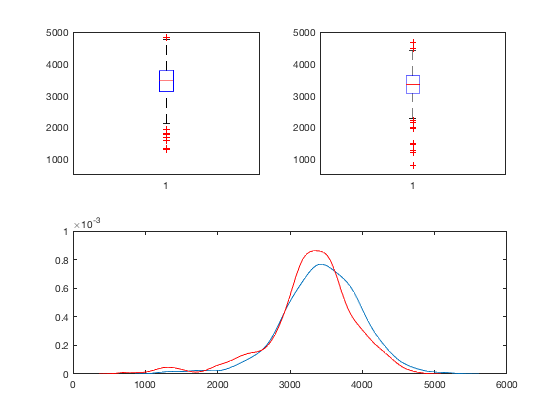
\includegraphics[width=10cm]{img/pb_5.png}\par
}

\begin{tcolorbox}
\textbf{Comments:}
the two box plots represent distribution of birth weight of children. The left one refers to a population whose mothers did smoke during the pregnancy while the right one refers to a population whose mothers did not smoke during the pregnancy. The box contains the median which is clearly lower in the second population. Also the minimum value is smaller in the second population, a sign of possible unhealthy children. In general from the lower plot is possible to see how the population with smoking mothers (red line) has a more scattered distribution with a bump in the right part of the plot.
\end{tcolorbox}
\end{document}


